\begin{abstract}
The peracarid taxon Cumacea is an essential indicator of benthic quality in marine ecosystems. This study investigated the influence of environmental (i.e., biological or ecosystemic), climatic (i.e., meteorological or atmospheric), and spatial (i.e., geographic or regional) variables on their genetic variability and adaptability in the Northern North Atlantic, focusing on Icelandic waters. We analyzed partial sequences of the 16S rRNA mitochondrial gene from 62 Cumacea specimens. Using the \textit{aPhyloGeo} software, we compared these sequences with relevant variables such as latitude (decimal degree) at the end of sampling, wind speed (m/s) at the start of sampling, O\textsubscript{2} concentration (mg/L), and depth (m) at the start of sampling.

Our analyses revealed variability in spatial and biological variables, reflecting the diversity of ecological requirements and benthic habitats. The most common Cumacea families, Diastylidae and Leuconidae, suggest adaptations to various marine environments. Phylogeographic analysis showed a divergence between specific genetic sequences and two habitat variables: wind speed (m/s) at the start of sampling and O\textsubscript{2} concentration (mg/L). This observation may indicate the possibility of varying local adaptations in response to these fluctuating conditions.

These results reinforce the importance of further research into the relationship between Cumacea genetics and global environmental variables to interpret the evolutionary dynamics and adaptation of these deep-sea organisms. This study sheds much-needed light on the acclimatization of invertebrates to climate change, anthropogenic pressures, and marine habitat management, potentially contributing to the evolution of more effective conservation strategies and policies to protect these vulnerable ecosystems.

The \textit{aPhyloGeo} Python package is freely and publicly available on \href{https://github.com/tahiri-lab/aPhyloGeo}{GitHub} and \href{https://pypi.org/project/aphylogeo/}{PyPi}, providing an invaluable tool for future research.
\end{abstract}

\section{Introduction}\label{introduction}
The North Atlantic and Subarctic regions, particularly the Icelandic waters, are of ecological interest due to their diverse water masses and unique oceanographic features \citep{schnurr_composition_2014, meisner_benthic_2014, uhlir_adding_2021}. These areas form vital {benthic habitats}\footnote{Areas at the bottom of oceans, lakes, or rivers, including sediments and organisms that live in them.} \citep{levin2009ecological} and enhance our understanding of deep-sea ecosystems and biodiversity patterns \citep{rogers2007corals, danovaro2008exponential, uhlir_adding_2021}. The IceAGE project and its predecessors, BIOFAR and BIOICE, provide invaluable data for studying the impacts of climate change and seabed mining, especially in the Greenland, Iceland, and Norwegian (GIN) seas \citep{meisner_prefacebiodiversity_2018}.

Cumacea, a crustacean taxon within Peracarida, are major indicators of marine ecosystem health due to their sensitivity to environmental fluctuations \citep{stransky_diversity_2010} and their contribution to benthic food webs \citep{rehm2009cumacea}. Despite their ecological importance, the evolutionary history of deep-sea benthic invertebrates remains uncharted, notably in the North Atlantic \citep{jennings_phylogeographic_2014}. Analyzing the genetic and distribution patterns of these deep-sea organisms is crucial for predicting their responses to climate change \citep{jennings_phylogeographic_2014} and anthropogenic pressures \citep{meisner_prefacebiodiversity_2018}, while also advancing our understanding of their adaptive mechanisms within deep-sea ecosystems.

Given the urgency of the aforementioned factors, this study aims to analyze the effects of ecological (climatic and environmental) and spatial variables on the genetic variation and adaptation of Cumacea in the Northern North Atlantic. More specifically, we will examine whether there is a genetic adaptation between the genetic structure of a region represented by a partial sequence of the 16S rRNA mitochondrial gene of the Cumacea species included in our analyses and their habitat variables. If so, we will identify which variables show the greatest divergence from a specific segment (i.e., window) of this partial sequence and further investigate the potential associated protein using bioinformatics tools to interpret its biological relevance. Our approach includes confirming various phylogeographic models\footnote{Phylogeographic models are computational tools that analyze relationships between the genetic structures of populations and their geographic distributions. In our case, by incorporating regional, biological, and atmospheric variables, we can analyze and interpret their impact on the genetic adaptation and spatial patterns of Cumacea species.} and updating a Python package (currently in beta), \textit{aPhyloGeo}, to facilitate these analyses.

This paper is organized as follows: \autoref{related-works} reviews pertinent studies on the biodiversity and biogeography of deep-sea benthic invertebrates; \autoref{contribution} summarizes the aims and contributions of this study, highlighting aspects relating to the conservation and adaptation of marine invertebrates to climate change; \autoref{materials-methods} describes data collection, preprocessing and phylogeographic analyses of partial genetic sequence and habitat variables; \autoref{metrics} describes the metrics used to evaluate the phylogeographic models; \autoref{results} presents the results; finally, \autoref{conclusion} discusses their implications for future research and conservation efforts.

\section{Related Works}\label{related-works}
Assessing and quantifying the biodiversity of deep-sea benthic invertebrates has become increasingly important since it was discovered that their species richness may be underestimated \citep{grassle1992deep}. Subsequent research has highlighted the need for large-scale distribution models to interpret the diversity of these organisms across their ecological and evolutionary contexts \citep{rex1997large}. Consequently, recent efforts have focused on mapping, managing, and studying the seabed \citep{brown2011benthic}. Advanced technologies, such as acoustic detection are improving our knowledge of benthic ecosystem complexity \citep{brown2011benthic}. Integrating genetic and habitat variables provides a better insight into how ecosystemic, meteorological, and spatial variables influence the genetic variation, distribution, biodiversity, and resilience of deep-sea benthic organisms \citep{vrijenhoek2009cryptic}.

However, the relationship between genetics and the environment is complex, involving gene-environment interactions and factors related to natural selection, which makes it difficult to identify clear causal relationships \citep{balkenhol_identifying_2009}. Additionally, the distinction between the direct and indirect effects of the environment on genetics presents further challenges \citep{manel_perspectives_2010, balkenhol_landscape_2019}. The limitations of current methods for measuring genetic and ecological variables, combined with logistical constraints, often limit the scope of such studies \citep{manel_perspectives_2010, shafer_widespread_2013}. This complexity may explain why the relationship between the environment and genetics of Cumacea has been less studied, despite their importance for understanding how deep-sea invertebrates adapt to fluctuating environmental conditions.

\section{Our Contribution}\label{contribution}
Our study focuses on the genetic fluctuation of a partial sequence of the 16S rRNA mitochondrial gene in Cumacea communities in response to variations in their habitat, a topic that has been little explored in previous studies \citep{grassle1992deep, rex2000latitudinal}. We aim to refine the natural selection hypothesis by identifying specific divergent genetic regions and the potentially associated proteins using bioinformatics tools, such as protein structure modeling and functional annotation databases, to reveal the potential functions that these proteins may have in the adaptation of Cumacea to habitat fluctuations. By linking this partial sequence to habitat variables using robust analytical methods, such as dissimilarity calculations and phylogenetic reconstructions, we can better interpret the selection effects at the molecular level of this Cumacea sequence, which could confer survival advantages in the harsh environments of the Northern North Atlantic. This represents a major advance over previous research, which has often struggled to integrate genetic and biological data in the context of deep-sea invertebrates \citep{etter1990population, vrijenhoek2009cryptic} or has faced difficulties in linking genetics and environment \citep{manel2003landscape, balkenhol2009statistical}.

Furthermore, our genetic and environmental data highlight habitats of high conservation interest that can be considered for establishing marine protected areas \citep{levin2009ecological}. These results are essential for developing informed conservation strategies in the context of climate change. Finally, our study paves the way for further research on other invertebrate species across different geographic regions. By extending this research to diverse environments and taxonomic groups, scientists will be better able to assess the adaptation and resilience of marine invertebrates to changing conditions.

\section{Materials and Methods}\label{materials-methods}
This section describes our data and introduces the main data preprocessing steps, the \textit{aPhyloGeo} software, the distance metrics used, and how the figures were created. A flow chart, constructed with the diagram software draw.io, summarizes this section (see Figure \ref{fig:fig1}).

\begin{figure}[htbp]
    \centering
    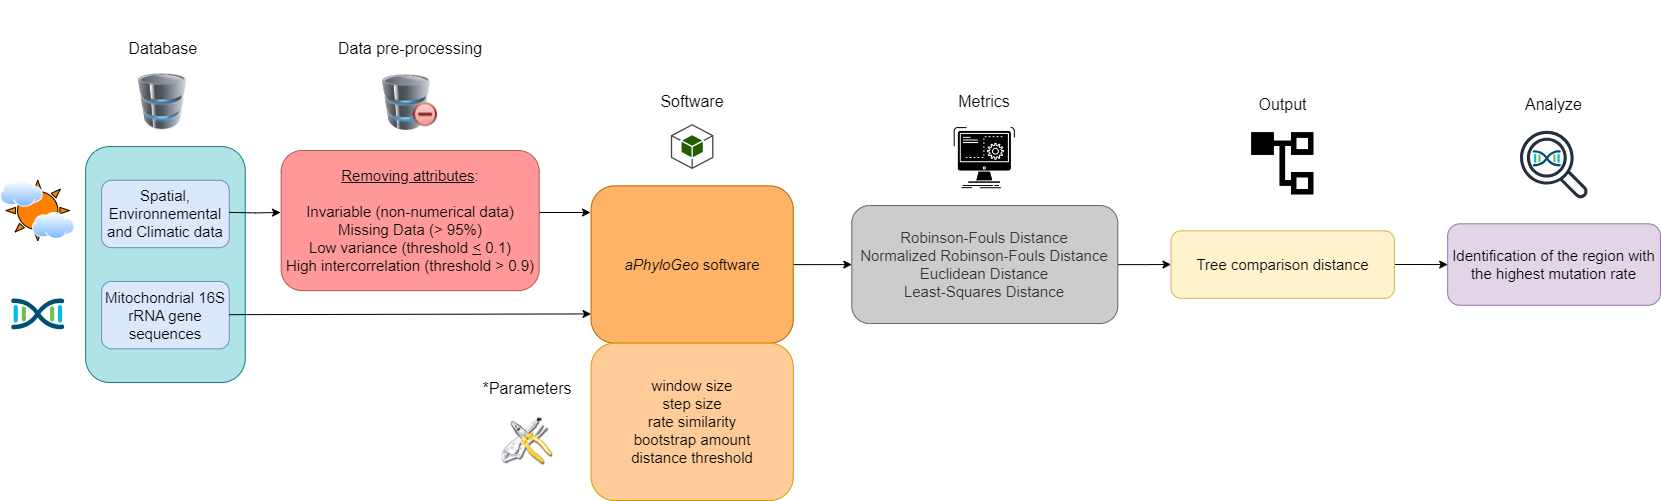
\includegraphics[width=0.7\textwidth]{diagram.drawio.png}
    \caption{Flow chart summarizing the Materials and Methods section workflow. Six different colors highlight the blocks. The first block (blue) represents our database. The second block (in red) is data preprocessing, which consists of deleting certain variables. The third and fourth blocks (orange) implement the \textit{aPhyloGeo} software and its parameters for our phylogeographic analyses. The fifth block (gray) applies distance metrics to the genetic and habitat variable trees produced. The sixth block (yellow) calculates and compares distance metrics between genetic and habitat variable trees. The seventh block (purple) identifies the most divergent habitat variables of a specific region of the partial sequence of the 16S rRNA mitochondrial gene based on the results of tree comparisons. *See YAML files on \href{https://github.com/tahiri-lab/aPhyloGeo}{GitHub} for more details on these parameters. \label{fig:fig1}}
\end{figure}

\subsection{Description of the data}
The study area is located in the Northern part of the North Atlantic, including the Denmark Strait, the Iceland Basin, the Irminger Basin, and the Norwegian Basin and Sea (see Figure \ref{fig:fig2}). The specimens analyzed were collected as part of the IceAGE project (Icelandic marine Animals: Genetic and Ecology; Cruise ship M85/3 in 2011), which focused on the deep continental slopes and abyssal waters around Iceland \citep{meisner_prefacebiodiversity_2018}. The sampling period for the included specimens was from August 30 to September 22, 2011, and they were collected at depths ranging from 315.9 m to 2567.7 m. Detailed protocols concerning the sampling plan, sample processing, DNA extraction steps, PCR amplification, sequencing, and aligned DNA sequences are available in \citep{uhlir_adding_2021}.

\begin{figure}[htbp]
    \centering
    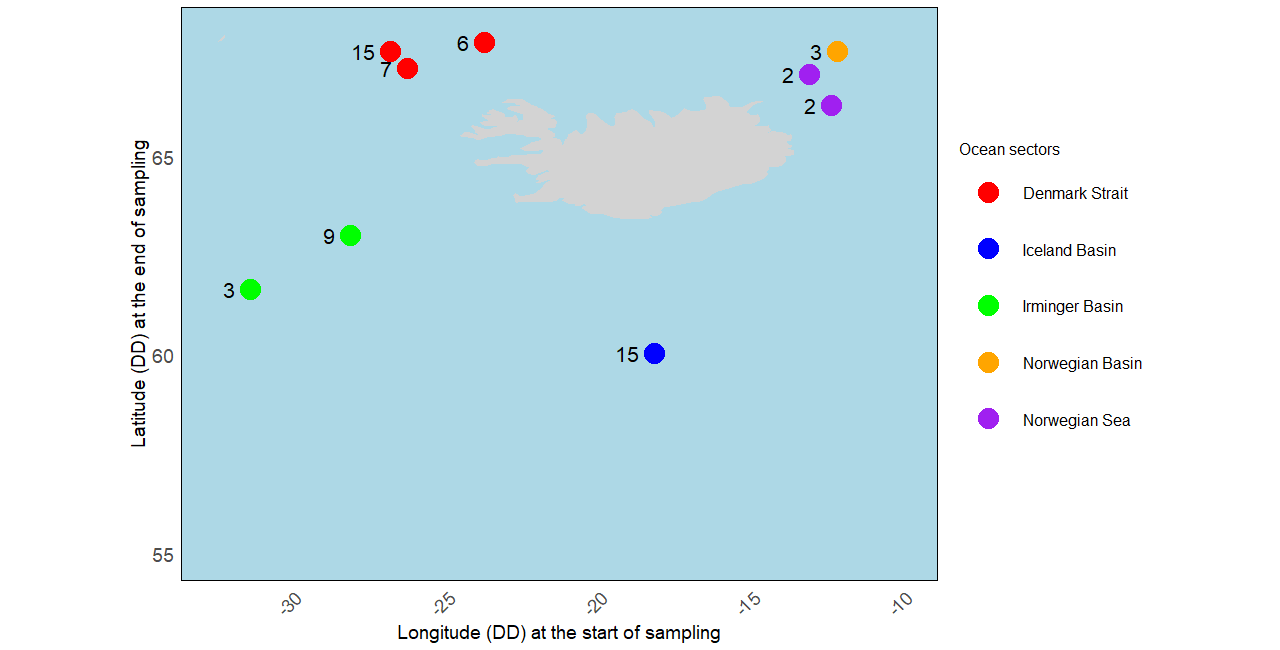
\includegraphics[width=0.7\textwidth]{figuremap.png}
    \caption{Distribution map of Cumacea specimens included in our analyses according to the oceanic sector where they were sampled. The grey area represents Iceland, and the number next to the point is the number of specimens found at that sampling point. \label{fig:fig2}}
\end{figure}

\subsection{Data preprocessing}
We used data from the article \citep{uhlir_adding_2021}, the IceAGE project, and related data from the BOLDSystem database, as described in \citep{uhlir_adding_2021}. Given these databases' enormous variety of variables, we applied a selective reduction procedure. Variables with no variability (categorical data) were excluded from our study, for which all data were missing and were not linked to genetic sequences or spatial, environmental, and climatic variables. Out of the 495 available in the IceAGE dataset, we considered 62 specimens for which partial 16S rRNA mitochondrial gene sequences were available.

Next, we calculated the variance ($S^2$) using the $var()$ function in RStudio Desktop 4.3.2 for each of the selected variables (numerical and categorical). This step aimed to eliminate variables with low variation, as they are unlikely to provide essential data for analysis. We set a variance threshold of ≤ 0.1 to exclude uninformative variables. The latter retains variables whose variability is reasonably sufficient for our analyses while rejecting those with little variation. Only water salinity was eliminated based on this criterion ($S^2\textsubscript{Salinity} = 0.02146629$). The formula (see Equation \ref{variance}) and code (\autoref{lst:variance}) used to calculate the variance of our final variables, available in the data file on \href{https://github.com/tahiri-lab/Cumacea_aPhyloGeo}{GitHub}, are provided below:

\begin{equation}\label{variance}
    S^2 = \frac{\sum_{i=1}^{n} (x_i - \bar{x})^2}{n-1}
\end{equation}

where $S^2$ is the variance of the variable, $x_i$ represents each value of the variable, $\bar{x}$ is the average of the values for this variable, and $n$ is the number of values for this variable in the dataset.

%\autoref{lst:variance}.
\begin{lstlisting}[label=lst:variance,language=R,caption=RStudio script to calculate the variance of each numerical and categorical variables in our final dataset.]
# Import data from the CSV file
Data <- read.csv(file="Final_Data_Article.csv", header=TRUE, sep=";")

# Define a function to calculate entropy for categorical variables
calculate_entropy <- function(x) {
  # Calculate the frequency of each category
  freq_table <- table(x)
  # Calculate probabilities
  probabilities <- freq_table / sum(freq_table)
  # Calculate entropy using the probabilities
  entropy_value <- -sum(probabilities*log(probabilities), na.rm=TRUE)
  return(entropy_value)
}

# Calculate variance
variances <- sapply(Data, function(x) {
  # Check if the column is numeric
  if (is.numeric(x)) {
    # Compute variance, excluding NA values
    var(x, na.rm=TRUE)
  } else if (is.factor(x) || is.character(x)) {
    # If the column is categorical, compute entropy
    calculate_entropy(x)
  } else {
    NA  # Return NA for other types of columns
  }
})

# Display variances/entropies
print(variances)
\end{lstlisting}

We calculated the Pearson correlation ($r$) between variables using the $cor()$ function in RStudio Desktop 4.3.2. Variables (numerical) exhibiting strong correlations with each other (threshold > 0.90) were removed to avoid repetition and guarantee variable independence. We considered the threshold of > 0.90 to be an adequate compromise between preserving properties for our analyses and eliminating the repetition of information in our data. Since we have three missing data for O\textsubscript{2} concentration (mg/L), we have used the "pairwise.complete.obs method". This method calculates the Pearson correlation matrix using all accessible pairs of observations, even if some data are missing. Using the above threshold, four variables were discarded: latitude (DD) at the start of sampling (Lat_start_end: $r = 0.9996658$), longitude (DD) at the end of sampling (Long_start_end: $r = 0.9999979$), depth (m) at the end of sampling (Depth_start_end: $r = 0.9998579$) and wind direction at the start of sampling (WindD_start_end: $r = 0.9752331$). The decision to remove these variables was based on their variance ($S^2$) value: $S^2\textsubscript{Lat_start} = 10.03077$ and $S^2\textsubscript{Lat_end} = 10.71335$; $S^2\textsubscript{Long_start} = 30.47940$ and $S^2\textsubscript{Long_end} = 30.47574$; $S^2\textsubscript{Depth_start} = 776437.1$ and $S^2\textsubscript{Depth_end = 775394.7$; $S^2\textsubscript{WindD_start} = 2.405077$ and $S^2\textsubscript{WindD_end} = 4.482285$. The formula (see Equation \ref{pearson}) and code (\autoref{lst:pearson}) used to calculate the Pearson correlation coefficient between our final numerical variables are shown below:

\begin{equation}\label{pearson}
    r = \frac{\sum_{i=1}^{n} (x_i - \bar{x})(y_i - \bar{y})}{\sqrt{\sum_{i=1}^{n} (x_i - \bar{x})^2 \sum_{i=1}^{n} (y_i - \bar{y})^2}}
\end{equation}

where $r$ is the Pearson correlation coefficient between two variables, $x_i$ are the values of the variable $x$, $y_i$ are the values of the variable $y$, $\bar{x}$ and $\bar{y}$ are respectively the averages of the two variables, and $n$ is the number of values of the two variables in the dataset.

%\autoref{lst:pearson}.
\begin{lstlisting}[label=lst:pearson,language=R,caption=RStudio script to calculate the Pearson correlation coefficient between all the numerical variables in our final dataset.]
# Import data
Data <- read.csv(file="Final_Data_Article.csv", header=TRUE, sep=";")

# Select numeric columns only from the dataset
numeric_Data <- Data[sapply(Data, is.numeric)]

# Calculate Pearson correlation matrix
correlation_matrix <- cor(numeric_Data, use="pairwise.complete.obs")

# Display correlation matrix
print(correlation_matrix)
\end{lstlisting}

This selection of variables and data resulted in a table containing 62 rows ($n=62$) and 16 columns (number of variables).

\subsection{Selected variables in the IceAGE database}
\subsubsection{Spatial data}
\begin{itemize}
\item The latitude at the end of sampling (see Figure \ref{fig:fig3}a) and longitude at the start of sampling (see Figure \ref{fig:fig3}b), both in decimal degrees (DD), as they are intimately linked to the environmental gradients and historical mechanisms modeling genetic heterogeneity \citep{gaither2013origins}.
\item The five oceanic sectors across the seas around Iceland (see Figure \ref{fig:fig2}): the Denmark Strait ($n=28$), the Iceland Basin ($n=15$), the Irminger Basin ($n=12$), the Norwegian Sea ($n=4$), and the Norwegian Basin ($n=3$).
\end{itemize}

\subsubsection{Environmental data}
\begin{itemize}
\item Depth (m) at the start of sampling (see Figure \ref{fig:fig3}c), as well as water temperature ($^\circ$C) (see Figure \ref{fig:fig3}e), and O\textsubscript{2} concentration (mg/L) (see Figure \ref{fig:fig3}f), as these are vital elements of the marine ecosystem that have an impact on the distribution and evolutionary acclimatization of marine species \citep{rex2006global, danovaro2010first}.
\item Since the sedimentary characteristics directly influence the distribution of Cumacea \citep{uhlir_adding_2021}, they were included in our data. They are divided into six ecological niche categories: mud ($n=30$), sandy mud ($n=15$), sand ($n=9$), forams ($n=3$), muddy sand ($n=3$), and gravel ($n=2$).
\end{itemize}

\subsubsection{Climatic data}
Wind speed (m/s) at the start (see figure \ref{fig:fig3}d) and end of sampling and wind direction at the end of sampling were also included, giving the contribution of wind to benthic ecosystem dynamics and the restructuring of species distribution by wind currents and sediment transport \citep{siedlecki2016experiments, waga_recent_2020,saeedi_environmental_2022}. The wind direction at the end of sampling comprises eight orientations: south (S, $n=15$), southwest (SW, $n=15$), northeast (NE, $n=9$), west-southwest (WSW, $n=7$), southeast (SE, $n=6$), north-northwest (NNW, $n=5$), south-southeast (SSE, $n=3$), and east (E, $n=2$).

\subsection{Selected variables in the BOLDSystem database}
\subsubsection{Taxonomic data}
The family, genus, and scientific name of the Cumacea were integrated into our data to study evolutionary relationships and genetic variation to habitat and acclimatization variables among the specimens. These comprise seven families (see Figure \ref{fig:fig4}): Diastylidae ($n=21$), Lampropidae ($n=13$), Leuconidae ($n=12$), Astacidae ($n=7$), Bodotriidae ($n=4$), Ceratocumatidae ($n=3$), and Pseudocumatidae ($n=2$). A total of 20 Cumacea species were included in our dataset (see Figure \ref{fig:fig4}). We have also included the sample identity (Sampleid) so that each specimen remains unique. Some specimens were only identified to family ($n=1$) or genus ($n=4$).

\subsection{Selected variables from article \cite{uhlir_adding_2021}}
\subsubsection{Other environmental data}
The habitat and water mass of the sampling points were the only environmental variables taken directly from Table 1 of \citep{uhlir_adding_2021}, as they can provide insight into how they may affect Cumacea genetic diversity and the acclimatization of these species in the GIN seas around Iceland. Thus, the water masses definitions, as described in \citep{uhlir_adding_2021}, were used as a reference: Arctic Polar Water (APW, $n=15$), Iceland Sea Overflow Water (ISOW, $n=15$), North Atlantic Water (NAW, $n=9$), warm Norwegian Sea Deep Water (NSDWw, $n=8$), Arctic Polar Water/Norwegian Sea Arctic Intermediate Water (APW/NSAIW, $n=7$), Labrador Sea Water (LSW, $n=3$), cold Norwegian Sea Deep Water (NSDWc, $n=3$), and Norwegian Sea Arctic Intermediate Water (NSAIW, $n=2$) (see Figure \ref{fig:fig5}). In terms of habitat, we considered the three categories used in \citep{uhlir_adding_2021}: Deep Sea ($n=38$), Shelf ($n=15$), and Slope ($n=9$) (see Figure \ref{fig:fig6}).

\subsubsection{Genetic data}
The aligned partial DNA sequence of the 16S rRNA mitochondrial gene was included, as this region is standard in phylogeny and phylogeography studies \citep{hugenholtz1998impact} and sufficiently conserved over time to guarantee exact alignments between different species \citep{saccone1999evolutionary}. We examined 61 of the 306 aligned DNA sequences used for phylogeographic analyses by \citep{uhlir_adding_2021}. As some specimens have their DNA sequence duplicated, or even quadruplicated with a difference of one or two nucleotides, the longest-aligned DNA sequence of each specimen was retained. The ``ICE1-Dia004'' specimen is the only one whose sequence (not aligned) was taken from the BoldSystem database, as it was absent from the \citep{uhlir_adding_2021} aligned DNA database.

\subsection{{\textit{aPhyloGeo} software}\label{aPhyloGeo-software}}
We used the cross-platform Python software \textit{aPhyloGeo}, developed by My-Linh Luu, Georges Marceau, David Beauchemin, and Nadia Tahiri, for our phylogeographic analyses. This software is designed to analyze phylogenetic trees using ecological and spatial variables (\autoref{lst:main}), to interpret the evolution of species under different environmental conditions \citep{koshkarov_phylogeography_2022}.

We selected this software for our analysis because, to our knowledge, it is the first phylogeographic tool capable of establishing similarity or dissimilarity between species genetics and environmental, climatic, and spatial variables \citep{koshkarov_phylogeography_2022} - precisely the objective of our study. The \textit{aPhyloGeo} software offers several key functionalities:

\begin{enumerate}[label=\arabic*.]
\item Phylogenetic tree evaluation: The software elucidates the evolutionary relationships between species based on their genetic sequences \citep{koshkarov_phylogeography_2022}, which is essential for interpreting phylogeographic models that link the evolution of species to their spatial distribution and their biological and meteorological context.
\item Ecological and regional dissimilarity analysis: It detects divergence and convergence between genetic sequences and habitat variables \citep{koshkarov_phylogeography_2022}, to identify the effect of these variables on the genetic fluctuations and evolutionary history of these Cumacea species.
\item Evaluation of genetic diversity: \textit{aPhyloGeo} measures genetic heterogeneity, making it possible to recognize potential evolutionary processes (e.g., mutation, speciation, and genetic drift) and local adaptations.
\end{enumerate}

%\autoref{lst:main}.
\begin{lstlisting}[label=lst:main,language=Python,caption=Main script for tutorial using the aPhyloGeo package.]
if __name__ == "__main__":

    # Load parameters
    Params.load_from_file(Params.reference_yaml_filepath)
    
    # Load the sequence file
    sequence_file = utils.loadSequenceFile(
                    Params.reference_gene_filepath)
    
    # Create an AlignSequences object
    align_sequence = AlignSequences(sequence_file)

    # Load variable data
    variable_data = pd.read_csv(Params.file_name)

    # Perform the alignment of sequences
    alignments = align_sequence.align()

    # Generate genetic trees based on aligned sequences
    geneticTrees = utils.geneticPipeline(alignments.msa)

    # Create a GeneticTrees object
    trees = GeneticTrees(trees_dict=geneticTrees, 
                        format="newick")

    # Generate variable trees
    variableTrees = utils.climaticPipeline(variable_data)

    # Filter the results based on the generated trees
    utils.filterResults(variableTrees, 
                       geneticTrees, 
                       variable_data)
\end{lstlisting}

The \textit{aPhyloGeo} Python package is freely and publicly available on \href{https://github.com/tahiri-lab/aPhyloGeo}{GitHub}, and is also available on \href{https://pypi.org/project/aphylogeo/}{PyPi}, to facilitate complex phylogeographic analyses. The software process has three main stages:

\begin{enumerate}
\item \textbf{The first step} was to collect DNA sequences from Cumacea of sufficient quality for the needs of our results \citep{koshkarov_phylogeography_2022}. In this study, 62 Cumacea specimens were selected to represent 62 partial sequences of the 16S rRNA mitochondrial gene. We then included, from our database, two climatic variables, namely wind speed (m/s) at the start and end of the sampling; three environmental variables, such as depth (m) at the start of sampling, water temperature ($^\circ$C), and O\textsubscript{2} concentration (mg/L); and two geographic variables, latitude (DD) at the end of sampling and longitude (DD) at the start of sampling.

\item \textbf{The second step} was to generate trees from genetic, biological, spatial, and meteorological data. For spatial variables, the {Neighbor-Joining method}\footnote{It is a method used to construct phylogenetic trees using distance matrices.} was applied between each pair of Cumacea from distinct spatial conditions to produce a symmetrical square matrix and build the spatial tree from this matrix \citep{koshkarov_phylogeography_2022}. Each geographic variable gives rise to a tree. If there are $m$ windows from the genetic sequences, there will be $m$ geographic trees. The same approach was applied to biological, meteorological, and genetic data.

For the genetic data, phylogenetic reconstruction was repeated to build genetic trees based on 62 partial sequences of the 16S rRNA mitochondrial gene, considering only data within a window that progresses along the alignment \citep{koshkarov_phylogeography_2022}. Each window in the alignment will give a genetic tree. If there are $n$ windows from the sequences, there will be $n$ phylogenetic trees. This displacement can vary according to the steps and the size of the window defined by the user (their length is determined by the number of base pairs (bp)) \citep{koshkarov_phylogeography_2022}.

In our case, we set up the \textit{aPhyloGeo} software as follows: $pairwiseAligner$ for sequence alignment; $\text{Hamming distance}$ to measure simple dissimilarities between sequences; $\text{Wider Fit by elongating with Gap (starAlignment)}$ algorithm takes alignment gaps into account, which is often mandatory in the case of major deletions or insertions in the sequences; $\text{windows\_size}$: 10 nucleotide (nt); and finally, $\text{step\_size}$: 1 nt. The last two configurations imply that for each 10 nt window, a phylogenetic tree is produced using the 10 nt sequence of each Cumacea. Next, the window is moved by 1 nt, creating a new tree with the next 10 nt, and so on until the end of the alignment. Genetic trees will be stored in an object called $T_1$, while spatial and ecological trees will be stored in another object called $T_2$.

\item \textbf{The third step} is to compare the genetic trees constructed in each sliding window with the ecosystemic, atmospheric, and regional trees using the Robinson-Foulds distance \citep{robinson_comparison_1981}, normalized Robinson-Foulds distance and Euclidean distance. These contribute to understanding the correspondence between Cumacea genetic sequences and their habitat variables. The approach also takes bootstrapping into account \citep{koshkarov_phylogeography_2022}. The results of these metrics were obtained using the functions $robinson\_foulds(tree1, tree2)$ and $euclidean\_dist(tree1, tree2)$ from the \textit{aPhyloGeo} software and were organized by the main function (\autoref{lst:main}). Those for the normalized Robinson-Foulds distance were obtained with the function $robinson\_foulds(tree1, tree2)$ (see the last line of code in \autoref{lst:robinsonFoulds}). The result of the metrics indicates which variables show the greatest genetic divergence according to the magnitude of the metric distances (see figures \ref{fig:fig7} and \ref{fig:fig8}).

A sliding-window approach enables the precise location of subtle sequences with high rates of genetic divergence \citep{koshkarov_phylogeography_2022}. This method involves moving a fixed-size window over the alignment of genetic sequences. This allows genetic trees to be built for each part of the aligned sequences, depending on the size of the window and the step size. It therefore makes it possible to recognize changes in evolutionary relationships along the partial sequence region of the 16S rRNA mitochondrial gene of Cumacea species. This method is essential to determine whether this region of the Cumacea genome can be affected by certain ecological or spatial variables in their habitat (see Figure \ref{fig:fig7} and Figure \ref{fig:fig8}).
\end{enumerate}

\subsection{Metrics}\label{metrics}
Our phylogeographic study used four distance measures to quantify differences between phylogenetic trees and habitat trees and assess dissimilarities between genetic sequences and our variables. This enables a comprehensive analysis of the evolutionary dynamics of Cumacea populations in different environmental contexts.

The following section presents a more concise version of the functions mentioned in the second and third steps of \autoref{aPhyloGeo-software}:

\subsubsection{Robinson-Foulds distance}\label{RF}
The Robinson-Foulds (RF) distance calculates the distance between phylogenetic trees built in each sliding window ($T_1$) and the variable trees ($T_2$) (see the list in the first step of the \autoref{aPhyloGeo-software}) \citep{tahiri2018new, koshkarov_phylogeography_2022}. This measurement is used to evaluate the topological differences between the two sets of trees (see Equation \eqref{eq:rf} and \autoref{lst:robinsonFoulds}).

For example, it evaluates the number of division differences between phylogenetic trees built within certain user-defined sliding windows (see the second step of the \autoref{aPhyloGeo-software}) and spatial trees built with latitude data (DD) at the end of sampling \citep{robinson_comparison_1981}. A high distance between a specific window and other windows considered in the RF distance analysis may imply that the habitat variable has little to no impact on the evolution of this particular DNA sequence and that the fluctuation of this variable might not explain the genetic divergences observed.

\begin{equation}\label{eq:rf}
    \text{RF}(T_1, T_2) = | \Sigma(T_1) \Delta \Sigma(T_2) |
\end{equation}

where $\text{RF}(T_1, T_2)$ is the Robinson-Foulds distance between the two sets of trees, $\Sigma(T_1)$ and $\Sigma(T_2)$ are the sets of divisions in trees $T_1$ and $T_2$ and $ \Delta $, the difference between these two sets.

%\autoref{lst:robinsonFoulds}.
\begin{lstlisting}[label=lst:robinsonFoulds,language=Python,caption=Python script for calculating the Robinson-Foulds Distance using the ete3 package in the aPhyloGeo package. The Newick format represents the phylogenetic and variable trees in text form.]
def robinson_foulds(tree1, tree2):

    # Initialize the Robinson-Foulds distance
    rf = 0
    
    # Convert trees from Newick format to ete3.Tree objects
    tree1_newick = ete3.Tree(tree1.format("newick"), format=1)
    tree2_newick = ete3.Tree(tree2.format("newick"), format=1)
    
    # Calculate the Robinson-Foulds distance
    rf, rf_max, common_leaves = tree1_newick.robinson_foulds(
                                tree2_newick, 
                                unrooted_trees=True)
                                
    # If there are no common leaves, set the RF distance to 0
    if len(common_leaves) == 0:
        rf = 0

    # Return the RF distance and its normalized value
    return rf, rf / rf_max
\end{lstlisting}

\subsubsection{Normalized Robinson-Foulds distance}\label{RFnorm}
The normalized Robinson-Foulds (nRF) distance scales the RF distance to account for the size variations in the trees (number of clades; i.e., a group of species with a common origin), allowing a more equitable comparison. It scales the distance to a range between 0 and 1. In our context, the distance has been normalized by $2n-6$, where $n$ represents the number of taxa (see Equation \eqref{eq:rf_norm} and the last line of code in \autoref{lst:robinsonFoulds}).

Since the size of environmental trees constructed with O\textsubscript{2} concentration data (mg/L) differs from that of other variables due to missing data, this nRF distance allows its dissimilarity with phylogenetic trees to be compared more fairly \citep{tahiri2018new, koshkarov_phylogeography_2022}. It reveals the relative influence of O\textsubscript{2} concentration (mg/L) on Cumacea phylogenetic relationships, independent of tree size \citep{tahiri2018new, koshkarov_phylogeography_2022}. A high value of this metric between a specific window and other windows considered in the nRF distance analysis suggests that we cannot conclude that there is a correlation between this DNA sequence and the variable. It may indicate a topological dissimilarity between the habitat variable tree and the gene trees at that position in the DNA sequence alignments.

\begin{equation}\label{eq:rf_norm}
    \text{RF}_{\text{norm}}(T_1, T_2) = \frac{| \Sigma(T_1) \Delta \Sigma(T_2) |}{| \Sigma(T_1) | + | \Sigma(T_2) |}
\end{equation}

where $ \text{RF}_{\text{norm}}(T_1, T_2)$ is the normalized Robinson-Foulds distance between the two sets of trees, $\Sigma(T_1)$ and $\Sigma(T_2)$ are the sets of divisions in trees $T_1$ and $T_2$ and $ \Delta $, the difference between these two sets.

\subsubsection{Euclidean distance}\label{euclidean}
In our study, the Euclidean distance calculates the distance between two sets of points in a multidimensional space, which designates the divisions of the two sets of trees ($T_1$ and $T_2$). It is used to compare divisions between two respective sets of trees to assess the degree of divergence or similarity of their topologies (see Equation \eqref{eq:euclidean} and \autoref{lst:euclideanDist}). Thus, their distance in the genetic trees and the habitat variable trees are compared for each pair of leaves.

By comparing the two sets of trees $T_1$ and $T_2$ using this metric, it is possible to measure the extent to which genetic divergences correspond to fluctuations in habitat variables. This is crucial for interpreting evolutionary relationships with these factors. A high distance of this metric between a specific window and other windows considered in the Euclidean distance analysis suggests evolutionary divergences between members of the Cumacea communities at the level of this DNA sequence and the variation of the habitat variable (see Figure \ref{fig:fig7}d and Figure \ref{fig:fig8}d). In other words, the habitat variable may not have a dominant contribution to the evolution of this specific sequence of Cumacea populations.

\begin{equation}\label{eq:euclidean}
    d_{\text{Euclidean}}(T_1, T_2) = \sqrt{\sum_{i=1}^{n} (T1_i - T2_i)^2}
\end{equation}

where $ d_{\text{Euclidean}}(T_1, T_2)$ is the Euclidean distance between the two sets of trees, and $T1_i$ and $T2_i$ represent the respective divisions of trees $T_1$ and $T_2$ for each i-th division.

%\autoref{lst:euclideanDist}.
\begin{lstlisting}[label=lst:euclideanDist,language=Python,caption=Python script for calculating the Euclidean distance using the ete3 and the dendropy packages in the aPhyloGeo package. The Newick format represents the phylogenetic and variable trees in text form.]
def euclidean_dist(tree1, tree2):

    # Initialize the Euclidean distance 
    ed = 0
    
    # Create a TaxonNamespace object to handle taxon information
    tns = dendropy.TaxonNamespace()

    # Load the first tree into a dendropy Tree object
    tree1_tc = dendropy.Tree.get(data=tree1.format("newick"),
                                 schema="newick",
                                 taxon_namespace=tns)

    # Load the second tree into a dendropy Tree object
    tree2_tc = dendropy.Tree.get(data=tree2.format("newick"),
                                 schema="newick",
                                 taxon_namespace=tns)

    # Encode the bipartitions of both trees
    tree1_tc.encode_bipartitions()
    tree2_tc.encode_bipartitions()

    # Calculate the Euclidean distance
    ed = dendropy.calculate.treecompare.euclidean_distance(
                                                 tree1_tc, 
                                                 tree2_tc)

    return ed
\end{lstlisting}

Interestingly, Euclidean distance is more sensitive to the subtle tree topology, making it suitable for identifying detailed correlations between genetic fluctuations and those of habitat variables \citep{czarna2006topology}. It can therefore be used to study fine divergences between trees, enabling nuanced identification of the effects of habitat variables on the genetic structure of species \citep{czarna2006topology}. As for the Robinson-Foulds distance (normalized or not), although widely applied in evolutionary biology, it is less sensitive to slight topological dissimilarities, making it less accurate for identifying fine correlations between genetics and habitat variables due to its structural nature \citep{smith2019bayesian, smith2020information}.

\subsection{Creating Figures}\label{Figures}
Figure \ref{fig:fig3}, Figure \ref{fig:fig4}, Figure \ref{fig:fig7} and Figure \ref{fig:fig8} were made with Python 3.11, while Figure \ref{fig:fig2}, Figure \ref{fig:fig5} and Figure \ref{fig:fig6} were made with RStudio Desktop 4.3.2.

\section{Results}\label{results}
The violin diagrams shown in Figure \ref{fig:fig3} are used to display summary statistics similar to box plots, showing medians (white lines), interquartile ranges (thickened black bars), and the rest of the distributions (thin black lines), except the ``extreme'' points. Wider areas indicate a greater probability of the variables taking a given value. They summarize the distribution of spatial (latitude at the end of sampling and longitude at the start of sampling, both in DD), atmospheric (wind speed (m/s) at the start of sampling), and ecosystemic (depth (m) at the start of sampling, water temperature ($^\circ$C), and O\textsubscript{2} concentration (mg/L)) data. These diagrams are essential for understanding habitat conditions and highlighting the variables that can potentially influence genetic fluctuation and adaptability in Cumacea. In Table \ref{fig:tab1} and Figure \ref{fig:fig3}, the variables are designated by their names from the IceAGE database, except for latitude (DD) at the end of sampling and longitude (DD) at the start of sampling, for which the term ``dec'' has been removed at the end to avoid confusion.

\begin{table}[ht]
\centering
\begin{tabular}{|l|l|c|c|c|c|c|c|}
\hline
\textbf{Attributes} & \textbf{Statistics} & \textbf{Mean} & \textbf{Std Dev} & \textbf{Q1} & \textbf{Median} & \textbf{Q3} & \textbf{Min} & \textbf{Max} \\ \hline
Lat end (DD)        &                     & 64.75         & 3.27             & 61.65       & 67.15           & 67.63       & 60.05        & 67.86        \\ \hline
Long start (DD)     &                     & -23.12        & 5.52             & -26.77      & -26.21          & -18.14      & -31.35       & -12.16       \\ \hline
Depth start (m)     &                     & 1412.57       & 881.16           & 579.10      & 1574.70         & 2504.70     & 315.90       & 2567.70      \\ \hline
Watertemp ground (°C) &                   & 1.45          & 1.73             & 0.07        & 0.71            & 2.65        & 0.85         & 4.28         \\ \hline
O2 saturation ground (mg/L) &             & 271.88        & 18.11            & 258.39      & 278.77          & 290.90      & 245.53       & 292.97       \\ \hline
Windspeed start (m/s) &                    & 6.26          & 2.16             & 5.25        & 6.00            & 7.00        & 2.00         & 11.00        \\ \hline
\end{tabular}
\caption{Table summarizing key statistics such as mean, median, standard deviation (Std Dev), 1st quartile (Q1) and 3rd quartile (Q3) of biological (depth (m) at the start of sampling, water temperature ($^\circ$C), and O\textsubscript{2} concentration (mg/L)), spatial (latitude (DD) at the end of sampling and longitude (DD) at the start of sampling) and atmospheric (wind speed (m/s) at the start of sampling) variables for our phylogeographic analyses. \label{fig:tab1}}
\end{table}

\begin{figure}[htbp]
    \centering
    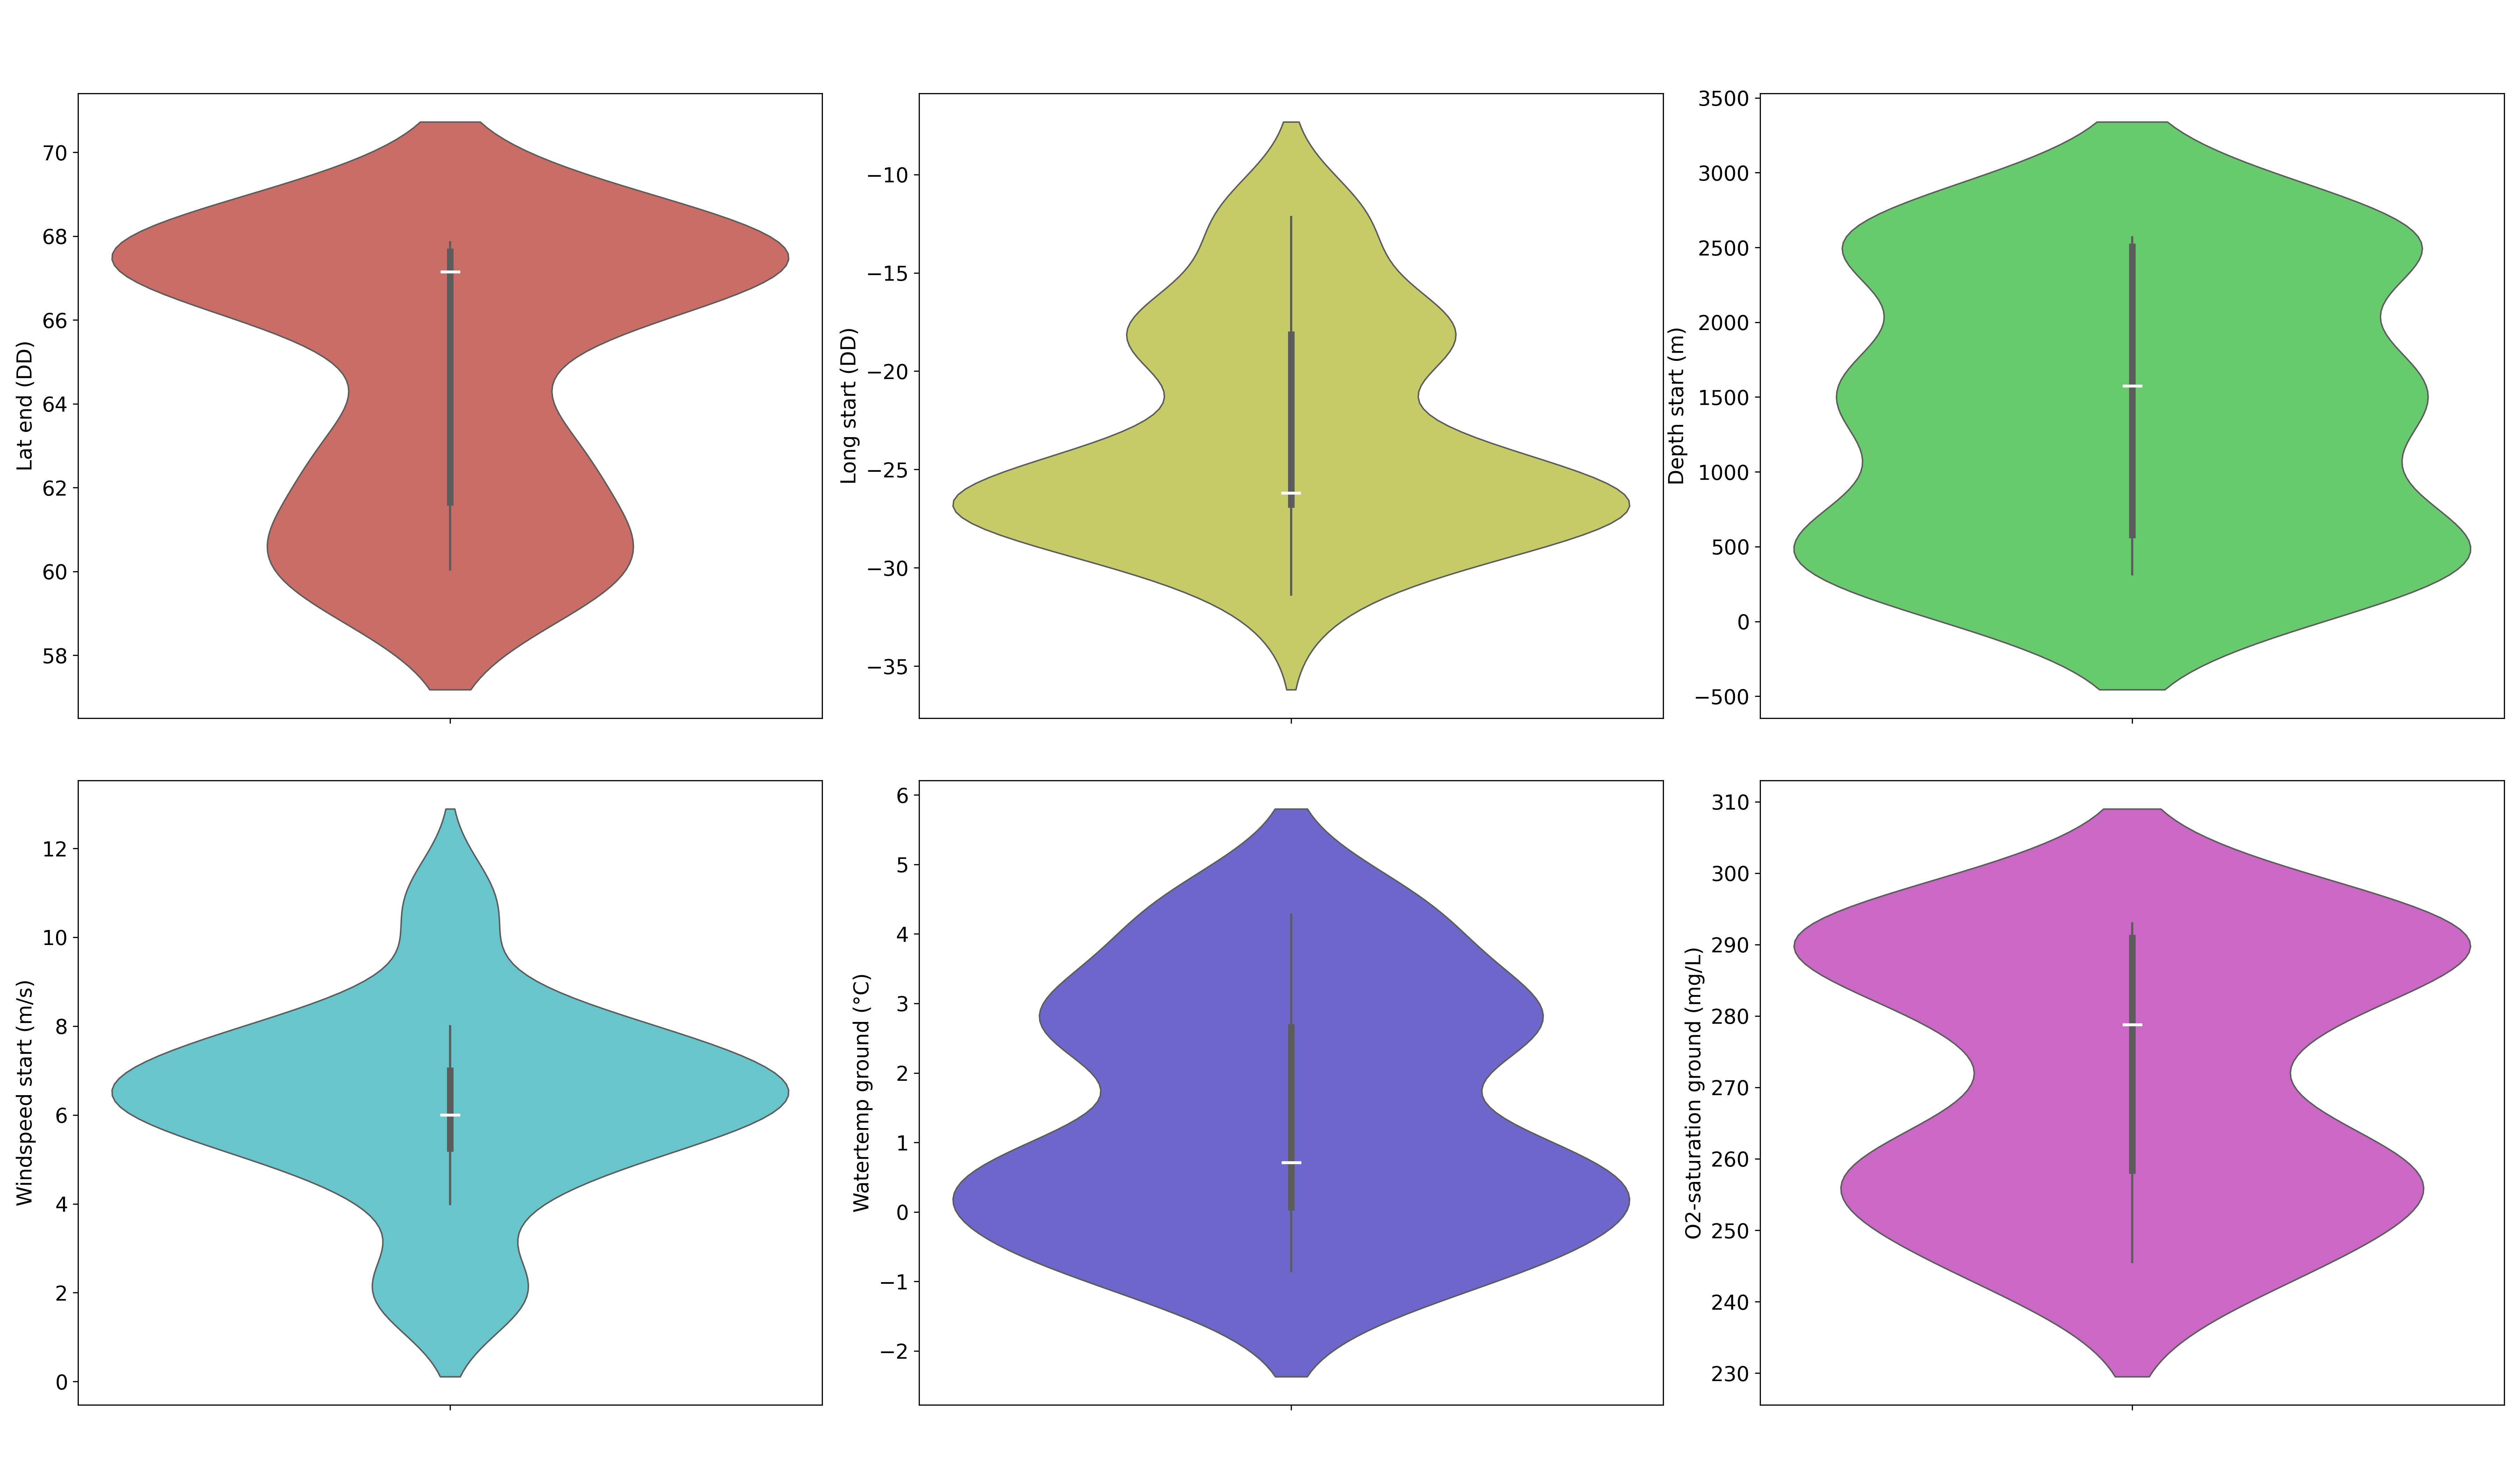
\includegraphics[width=0.7\textwidth]{figure1.jpg}
    \caption{Violin diagrams of two regional, one atmospheric, and three ecosystemic variables that provide essential information about the ecological and meteorological conditions of Cumacea habitats. a) Latitude (DD) at the end of sampling (red) suggest that the specimens come from two dominant latitudinal (DD) regions (around 61.65 DD and 67.63 DD); b) Longitude (DD) at the start of sampling (yellow) implies that the specimens come from two dominant longitudinal (DD) regions (around -26.77 DD and -18.14 DD); c) Depth (m) at the start of sampling (green) suggest that the specimens were mainly collected and concentrated at three different depths (m) (around 500 m, 1500 m and 2500 m); d) Wind speed (m/s) at start of sampling (light blue) indicate stable the wind conditions (m/s) at the start of sampling (around 6.00 m/s); e) Water temperature ($^\circ$C) (dark blue) suggest that the specimens were mostly collected and concentrated at two different water temperatures ($^\circ$C) (around 0.07 $^\circ$C and 2.66 $^\circ$C); f) O\textsubscript{2} concentration (mg/L) (pink) implies that the specimens were primarily collected and concentrated at two different O\textsubscript{2} concentrations (mg/L) (around 258.39 mg/L and 290.90 mg/L). \label{fig:fig3}}
\end{figure}

Our results revealed variability in most habitat variables, as shown in Figure \ref{fig:fig3}. For instance, the median of the latitude at the end of sampling (67.15 DD; Table \ref{fig:tab1}) is higher than the mean (64.75 DD; Table \ref{fig:tab1}), showing an asymmetric distribution skewed towards lower values. This trend is also observed for depth (m) at the start of sampling (Median: 1574.70 m; Mean: 1412.57 m; see Figure \ref{fig:fig3}c and Table \ref{fig:tab1}) and O\textsubscript{2} concentration (mg/L) (Median: 278.77 mg/L; Mean: 271.88 mg/L; see Figure \ref{fig:fig3}f and Table \ref{fig:tab1}). The bimodal shape of the latitude distribution curve suggests that the specimens came from two dominant latitudinal regions at the end of sampling (around 61.65 DD and 67.63 DD; see Figure \ref{fig:fig3}a and Table \ref{fig:tab1}). This bimodality is also observed in longitude (DD) at the start of sampling (around -26.77 DD and -18.14 DD; see Figure \ref{fig:fig3}b and Table \ref{fig:tab1}), as well as for water temperature ($^\circ$C) (around 0.07 $^\circ$C and 2.66 $^\circ$C; see Figure \ref{fig:fig3}e and Table \ref{fig:tab1}), and O\textsubscript{2} concentration (mg/L) (around 258.39 mg/L and 290.90 mg/L; see Figure \ref{fig:fig3}f and Table \ref{fig:tab1}).

The median of the longitude (DD) at the start of sampling (-26.21 DD; Table \ref{fig:tab1}) is lower than the mean (-23.12 DD; Table \ref{fig:tab1}), indicating asymmetry on the higher sides (see Figure \ref{fig:fig3}b), as does the water temperature ($^\circ$C) (Mean: 1.45 $^\circ$C; Median: 0.71 $^\circ$C; see Figure \ref{fig:fig3}e and Table \ref{fig:tab1}). Unlike all the other diagrams in Figure \ref{fig:fig3}, the curve of the depth (m) at the start of sampling (see Figure \ref{fig:fig3}c) has a multimodal shape with three prominent peaks, suggesting that the specimens were mainly collected and concentrated at three different depths (around 500 m, 1500 m and 2500 m; see Figure \ref{fig:fig3}c).

The mean (6.26 m/s; Table \ref{fig:tab1}) and median of wind speed (m/s) at the start of sampling are fairly similar, with a high density of data around the median (6.00 m/s; see Figure \ref{fig:fig3}d and Table \ref{fig:tab1}). This suggests stable wind conditions (m/s) at the start of sampling. The key statistics and the figure for the wind speed (m/s) at the end of sampling are available in the $img$ file on \href{https://github.com/tahiri-lab/Cumacea_aPhyloGeo}{GitHub}. The standard deviation of water temperature ($^\circ$C) is relatively high (1.73 $^\circ$C; Table \ref{fig:tab1}) compared to the mean (1.45 $^\circ$C; Table \ref{fig:tab1}), suggesting acclimatization of Cumacea to a variety of habitat temperatures (-0.85 $^\circ$C – 4.28 $^\circ$C; see Figure \ref{fig:fig3}e and Table \ref{fig:tab1}). The range of data for O\textsubscript{2} concentration (mg/L) shows some variability (245.53 mg/L – 292.97 mg/L; see Figure \ref{fig:fig3}f and Table \ref{fig:tab1}) in the environmental conditions. This reflects a diversity of requirements in terms of O\textsubscript{2} concentration (mg/L), with Cumacea potentially affected by the heterogeneity of biogeochemical cycles, such as photosynthesis, respiration, and organic decomposition, which affect depth-dependent dissolved O\textsubscript{2} concentration (mg/L).

\begin{figure}[htbp]
    \centering
    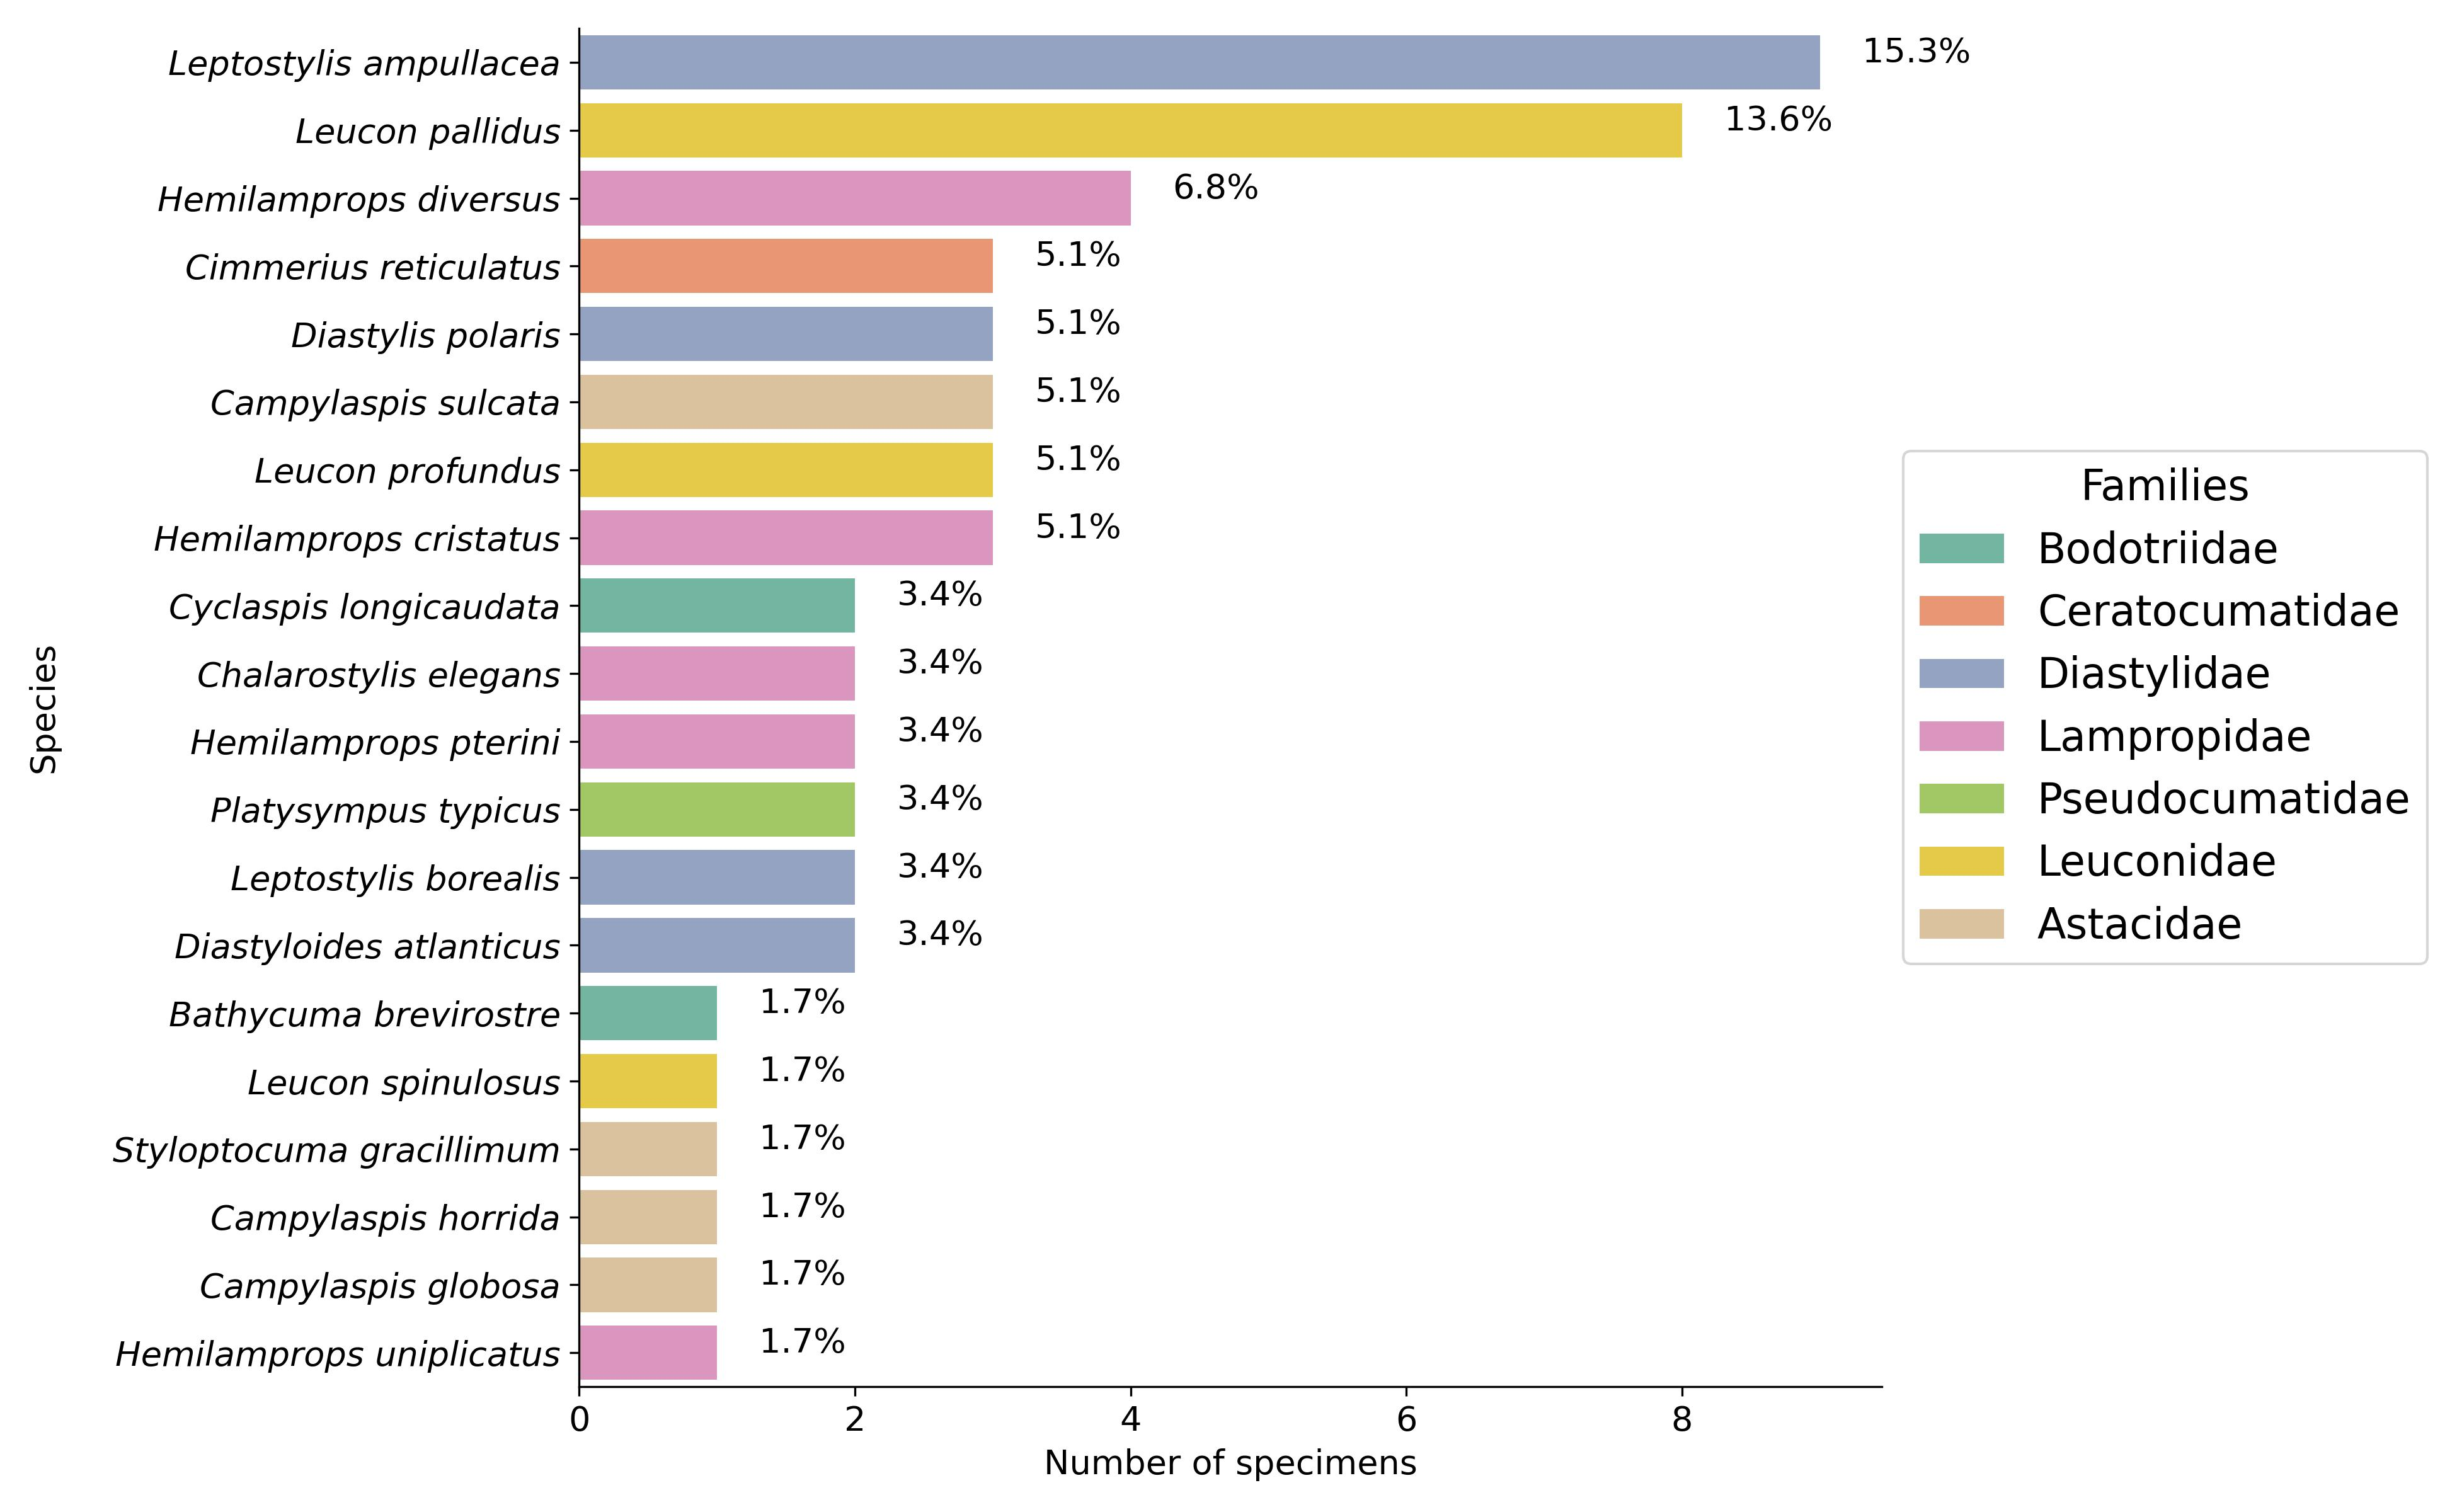
\includegraphics[width=0.7\textwidth]{figure2.jpg}
    \caption{Cumacea frequency distribution by species and family. The percentages (\%) displayed above the bars indicate the relative abundance of each species in our dataset. Unlike less common species, those that are abundant (such as \emph{Leptostylis ampullacea} and \emph{Leucon pallidus}) may have adaptive characteristics that enable them to exploit resources more easily, resist interspecific competition or withstand changing biological conditions. \label{fig:fig4}}
\end{figure}

The distribution and diversity of the various Cumacea species and family found are shown in Figure \ref{fig:fig4}. It shows that the most represented species are \emph{Leptostylis ampullacea} (14.1\%) and \emph{Leucon pallidus} (12.5\%). In contrast, species like \emph{Bathycuma brevirostre} and \emph{Styloptocuma gracillimum} are less represented (1.6\%), implying that some species may have restricted ecological niches or face ecological forces that limit their distribution. The dominance of certain species (such as \emph{Leptostylis ampullacea} and \emph{Leucon pallidus}) suggests that they may have adaptive traits that enable them to make the most of the accessible resources, resist interspecific competition, or survive in fluctuating ecosystemic conditions, aligns with our study’s aim of relating genetic adaptation to habitat characteristics.

\begin{figure}[htbp]
    \centering
    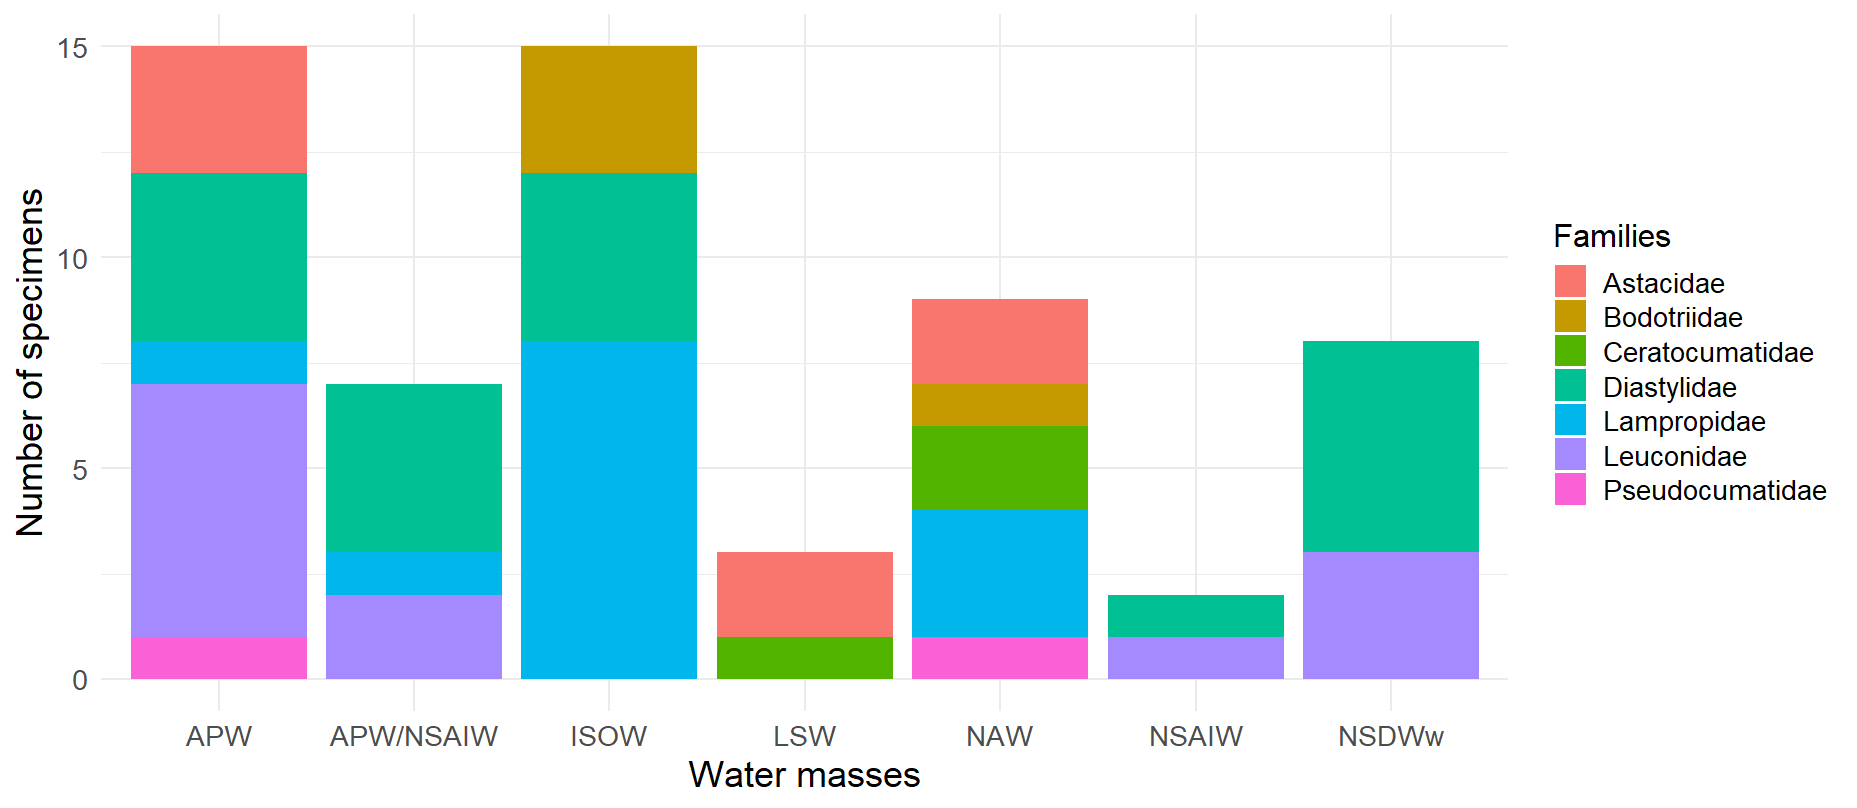
\includegraphics[width=0.7\textwidth]{figure3.png}
    \caption{Distribution of Cumacea families by water mass. This histogram represents the frequency of occurrence of the different Cumacea families, classified according to the water mass in which they were collected. Eight water mass categories are represented: Arctic Polar Water (APW), Arctic Polar Water/North Sub-Arctic Intermediate Water (APW/NSAIW), Iceland Scotland Overflow Water (ISOW), Labrador Sea Water (LSW), North Atlantic Water (NAW), North Sub-Arctic Intermediate Water (NSAIW), cold North Sub-Atlantic Deep Water (NSDWc), and warm North Sub-Atlantic Deep Water (NSDWw). The presence of the Diastylidae (turquoise) family in the majority of water bodies (APW, APW/NSAIW, ISOW, NSAIW, NSDWc, and NSDWw) accentuates the resilience and ecological acclimatization of this family to various ecological niches and conditions. \label{fig:fig5}}
\end{figure}

The figure above supports the objective of our study by showing the distribution of the different Cumacea families in the various water masses (see Figure \ref{fig:fig5}). The Diastylidae family, for example, is the most common in all water masses (turquoise color in Figure \ref{fig:fig5}), testifying to its resilience and ecological adaptability to a wide variety of habitat conditions, reminiscent of the dominance of \emph{Leptostylis ampullacea} which belongs to the Diastylidae family (see Figure \ref{fig:fig4}, 14.1\%).

\begin{figure}[]
    \centering
    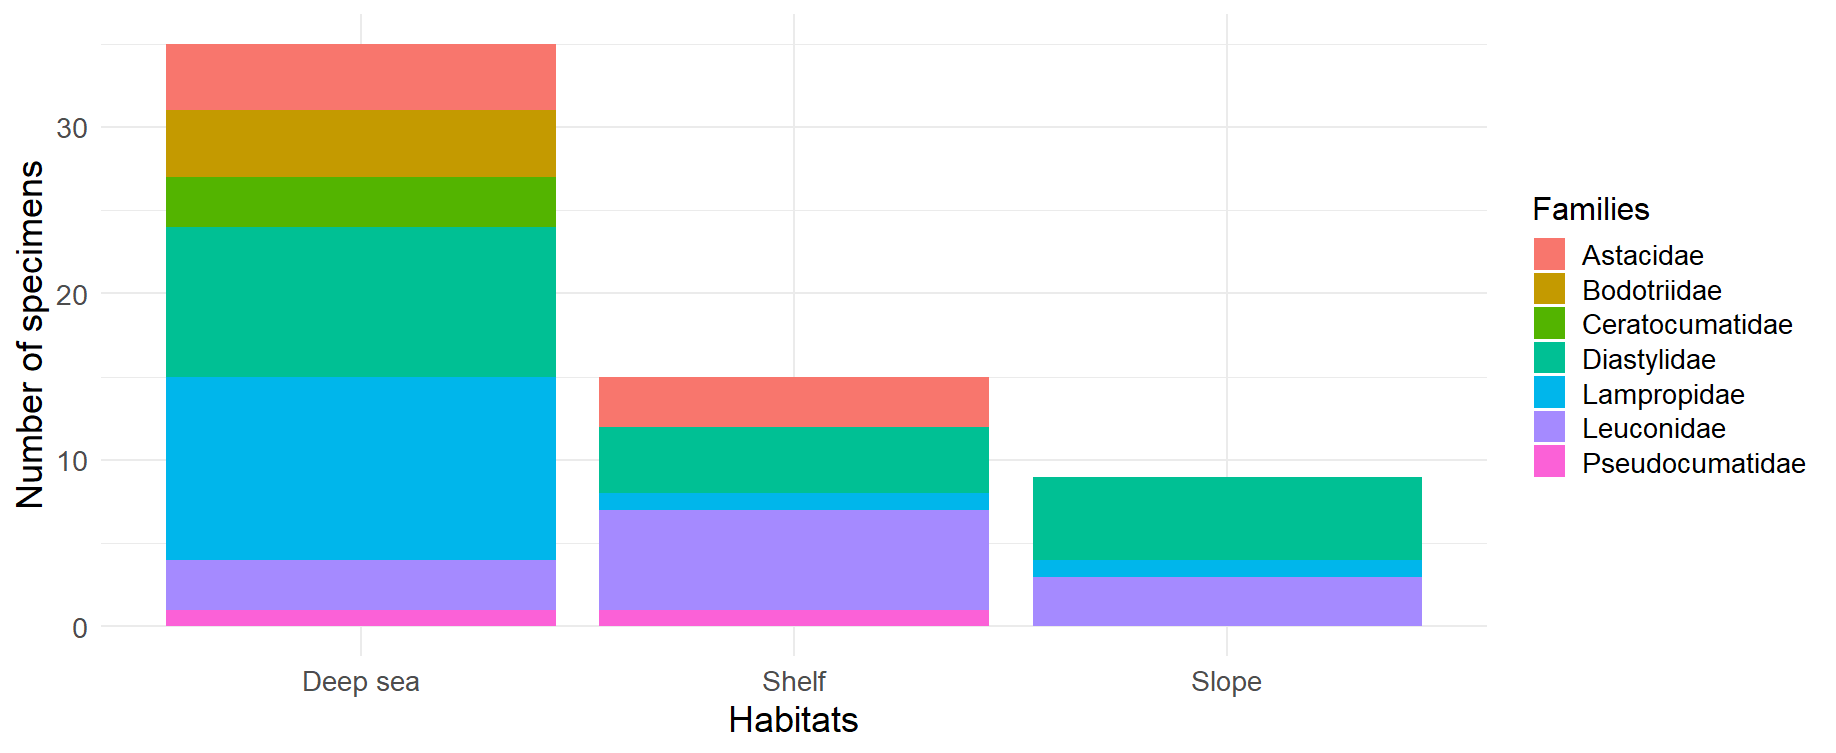
\includegraphics[width=0.7\textwidth]{figure4.png}
    \caption{Distribution of Cumacea families by habitat. This histogram represents the frequency of occurrence of the different Cumacea families, classified according to the habitat in which they were collected. Three habitat categories are represented: Deep Sea, Shelf, and Slope. The presence of Cumacea families in more than one habitat, such as Diastylidae (turquoise), Lampropidae (blue), Leuconidae (purple), Pseudocumatidae (pink), and Astacidae (red), may indicate the development of adaptations, whether morphological, physiological or behavioral, that could favor their persistence in these habitats. \label{fig:fig6}}
\end{figure}

The distribution of the different Cumacea families according to the type of habitat where they were collected during sampling is shown in Figure \ref{fig:fig6}. The deep-sea habitats show the greatest diversity of families, mainly Diastylidae and Lampropidae, suggesting they are well acclimatized to deep-sea conditions. In contrast, the slope has the lowest diversity, with Diastylidae again the most dominant, implying that some Cumacea species have fewer ecological niches or are less adapted to this habitat. Although less diverse than the deep sea, the shelf is dominated by Leuconidae, indicating that this family may be specifically well-acclimated to this habitat. These patterns imply that certain Cumacea families, such as the Diastylidae, Lampropidae, Leuconidae, Pseudocumatidae, and Astacidae, have developed distinct adaptations (physiological, behavioral, or morphological) to remain in particular ecological niches, reflecting the impact of habitat conditions on the genetic distribution of Cumacea.

\begin{figure}[]
    \centering
    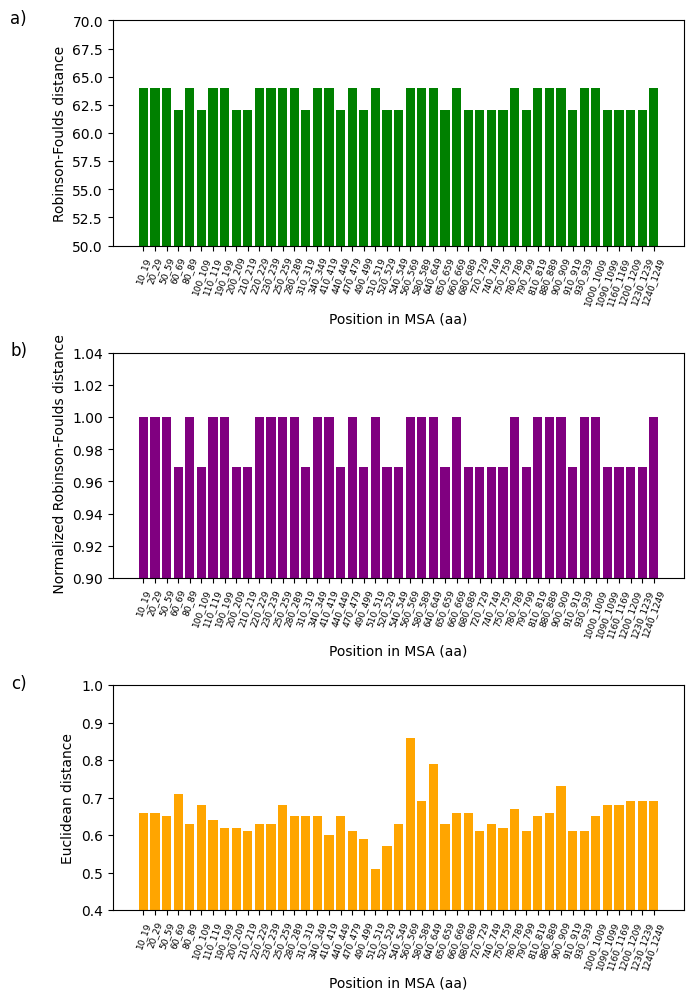
\includegraphics[width=0.7\textwidth]{figure5.png}
     \caption{Analysis of fluctuations in three distance metrics using multiple sequence alignment (MSA): a) Robinson-Foulds distance, b) normalized Robinson-Foulds distance, and c) Euclidean distance. Distance variations are studied to establish the potential dissimilarity between the partial sequence of the 16S rRNA mitochondrial gene of 62 Cumacea specimens and the variability of wind speed (m/s) at the start of sampling. \label{fig:fig7}}
\end{figure}

\begin{figure}[]
    \centering
    
\includegraphics[width=0.7\textwidth]{figure6.png}
    \caption{Analysis of fluctuations in three distance metrics using multiple sequence alignment (MSA): a) Robinson-Foulds distance, b) normalized Robinson-Foulds distance, and c) Euclidean distance. These distances aim to determine the degree of dissimilarity between the partial sequence of the 16S rRNA mitochondrial gene of 62 Cumacea specimens and the variation in O\textsubscript{2} concentration (mg/L) at the sampling sites. \label{fig:fig8}}
\end{figure}

The divergence between the genetic sequences and two variables, one climatic (wind speed (m/s) at the start of sampling) and the other environmental (O\textsubscript{2} concentration (mg/L)) is presented in Figure \ref{fig:fig7} and Figure \ref{fig:fig8}. All the variables given in the first step of the \autoref{aPhyloGeo-software} section were analyzed and their figures are available in the $img$ file on \href{https://github.com/tahiri-lab/Cumacea_aPhyloGeo}{GitHub}. However, only these two show the most interesting rate of divergence. Using the three metrics mentioned in the \autoref{metrics}, we noticed that the Euclidean distance is particularly sensitive to our data, manifesting considerable sequence variation at the position in MSA 560-569 amino acids (aa) (Euclidean distance: 0.86; see Figure \ref{fig:fig7}d) and 1210-1219 aa (Euclidean distance: 1.23; see Figure \ref{fig:fig8}d). Unlike the other windows for this metric in the two figures (see Figure \ref{fig:fig7}d and Figure \ref{fig:fig8}d), the fluctuations in wind speed (m/s) at the start of sampling and in O\textsubscript{2} concentration (mg/L) do not appear to explain the variations in these two specific sequences. This could indicate the absence of directional selection in these sequences due to these habitat variables, local selective pressures not considered in our analysis, or other evolutionary factors (e.g., genetic drift or biotic interactions) predominate over these two variables concerning these two sequences. On the other hand, this may suggest that these two variables could potentially influence the divergent (i.e., genetic diversification) rather than a convergent adaptation of these Cumacea, reflecting unique evolutionary responses to these specific ecological pressures. These results are consistent with the aim of our study, which is to identify the Cumacea genetic region that diverges most as a function of habitat variables, to determine whether this is due to divergent local adaptation or other evolutionary processes.

These results provide important insight into the genetic adaptation of Cumacea to their environment. These results need to be analyzed in greater depth to certify their involvement, especially in contrast with \citep{uhlir_adding_2021}, which investigated similar topics of environmental and climatic effects on Cumacea distribution and genetics. The \textit{aPhyloGeo} package is still in the process of being updated.

\section{Conclusion}\label{conclusion}
This study examines the effects of meteorological, regional, and ecosystemic variables on the genetics of Cumacea in the waters surrounding Iceland. Our main objective is to determine whether there is a discrepancy between the precise genetic information of the partial 16S rRNA mitochondrial gene sequence (i.e. a window) of Cumacea species and their habitat variables. In addition to data distribution representations (see Figure \ref{fig:fig3}, Figure \ref{fig:fig4}, Figure \ref{fig:fig5} and Figure \ref{fig:fig6}), DNA sequence analyses have identified specific genetic windows that diverge from atmospheric and biological variables such as wind speed (m/s) at the start of sampling (Position in MSA: 560-569 aa; Euclidean distance: 0.86; see Figure \ref{fig:fig7}d) and O\textsubscript{2} concentration (mg/L) (Position in MSA: 1210-1219 aa; Euclidean distance: 1.23; see Figure \ref{fig:fig8}d). These results could mean that these specimens have been shaped by these unique local environments, resulting in genetic sequences adapted to their particular conditions.

The novelty in our research lies in the exhaustive divergence between habitat variables and genetic mutability in Cumacea, particularly in identifying genetic windows associated with habitat fluctuations, which has not been widely investigated in previous studies \citep{manel2003landscape, vrijenhoek2009cryptic}. In this case, our integrated method identifies specific genetic regions sensitive to ecosystemic and atmospheric variations. Thus, by seeking to determine which of these two variables diverges most with the DNA sequences, the eventual identification of proteins linked to one of these variable DNA sequences will make it possible to represent its functional effects in responses to habitat changes. Our future research will focus on verifying the prediction of this protein and assessing its role in the physiological adaptation of Cumacea to fluctuating conditions, adding a link between genetic data and ecological function.

Interpreting how marine invertebrates genetically adapt to variations in their habitat can help predict their response to climate change and advance conservation plans to protect them. Identifying the specific variables that influence genetic variability in Cumacea can contribute to the designation and supervision of marine protected areas, assuring they include habitats crucial to the survival and acclimatization of these species. Thus, our results can inform the management of fishing and seabed mining companies by revealing ecologically vulnerable areas where these disturbances can seriously affect benthic biodiversity.

Furthermore, our results provide essential knowledge to guide future studies on the genetic adaptation of Cumacea and other invertebrates to ecological and regional variability. Based on these findings, future research should focus on additional ecosystemic and meteorological variables, such as nutrient accessibility, water pH, ocean currents, and the degree of human disturbance, to further improve the interpretation of the complex interactions between genetics and the environment. Extending the scope of application to other marine species, not just marine invertebrates, and various spatial regions would provide a better means of generalizing the results. With this in mind, longitudinal study models on these species could reflect long-term climatic and biological fluctuations and improve our knowledge of the dynamics of genetic acclimatization.

However, it is important to recognize the limitations of our study. In particular, the three missing data points on O\textsubscript{2} concentration (mg/L) and the relatively small sample size ($n=62$) may have induced a bias, which could impact the validity of our interpretations and restrict the generalizability of our results. Moreover, these missing data could provide partial insight into the relationship between O\textsubscript{2} concentration (mg/L) and genetic fluctuation in Cumacea, and our sample size may reduce the statistical power of our results. Future studies should address these gaps by incorporating larger sample sizes and more complete datasets to confirm and expand our conclusions. Additionally, as our research focuses solely on the partial sequence of the mitochondrial 16S rRNA gene, utilizing more elaborate genomic methods, such as whole-gene or even whole-genome sequencing, could help better understand marine species' genetic variety and global acclimatization mechanisms. This would provide more comprehensive genetic databases to improve our accuracy and knowledge in identifying existing (and new) marine invertebrate species using DNA barcoding (e.g., mitochondrial DNA cytochrome c oxidase I (COX1)). Finally, multidisciplinary collaborations between ecology, genetics, and oceanography would be essential to enhance knowledge sharing and its application in future research.

\section{Acknowledgments}\label{acknowledgments}
The authors thank the SciPy conference and reviewers for their valuable comments on this paper as well as Mansour Kebe for his technical support and Carolin Uhlir for her clarifications and advice on her study \citep{uhlir_adding_2021}. This work was supported by the Natural Sciences and Engineering Research Council of Canada (NSERC), the Fonds de recherche du Québec - Nature et technologies (FRQNT), the Université de Sherbrooke grant, and the Centre de recherche en écologie de l’Université de Sherbrooke (CREUS).
